\documentclass{article}


% if you need to pass options to natbib, use, e.g.:
%     \PassOptionsToPackage{numbers, compress}{natbib}
% before loading neurips_2023


% ready for submission
% \usepackage{neurips_2023}


% to compile a preprint version, e.g., for submission to arXiv, add add the
% [preprint] option:
  \usepackage[preprint]{neurips_2023}


% to compile a camera-ready version, add the [final] option, e.g.:
  % \usepackage[final]{neurips_2023}


% to avoid loading the natbib package, add option nonatbib:
  %  \usepackage[nonatbib]{neurips_2023}


\usepackage[utf8]{inputenc} % allow utf-8 input
\usepackage[T1]{fontenc}    % use 8-bit T1 fonts
\usepackage{hyperref}       % hyperlinks
\usepackage{url}            % simple URL typesetting
\usepackage{booktabs}       % professional-quality tables
\usepackage{amsfonts}       % blackboard math symbols
\usepackage{nicefrac}       % compact symbols for 1/2, etc.
\usepackage{microtype}      % microtypography
\usepackage{xcolor}         % colors
\usepackage{graphicx}       % Required for including graphics
\usepackage{subcaption}     % Required for subfigure environment
\usepackage{listings}       % Required for lstlisting environment
\usepackage{float}          % Enables tables to be rendered anywhere on the page
\usepackage{amsmath}        % For math environments like equation
\usepackage{pgfplots}       % For histogram
\usepackage{tikz}           % For histogram
\pgfplotsset{compat=1.18}


\title{BME1312 Project2 Report: Deep Learning Cardiac Cine MRI Segmentation}


% The \author macro works with any number of authors. There are two commands
% used to separate the names and addresses of multiple authors: \And and \AND.
%
% Using \And between authors leaves it to LaTeX to determine where to break the
% lines. Using \AND forces a line break at that point. So, if LaTeX puts 3 of 4
% authors names on the first line, and the last on the second line, try using
% \AND instead of \And before the third author name.


\author{%
  Wenye Xiong \\
  2023533141 \\
  \texttt{xiongwy2023@shanghaitech.edu.cn}
  \And
  Renyi Yang \\
  2023533030 \\
  \texttt{yangry2023@shanghaitech.edu.cn}
  \AND
  Jiaxing Wu \\
  2023533160 \\
  \texttt{wujx2023@shanghaitech.edu.cn}
  \And
  Boyang Xia \\
  2023533073 \\
  \texttt{xiaby2023@shanghaitech.edu.cn}
  \AND
  Fengmin Yang \\
  2023533183 \\
  \texttt{yangfm2023@shanghaitech.edu.cn}
}

\begin{document}


\maketitle


\begin{abstract}
  This report details the implementation and evaluation of U-Net based deep learning models for cardiac segmentation
  in cine MRI scans. The project focuses on segmenting three key structures: the Left Ventricle (LV), Right Ventricle (RV),
  and Myocardium (MYO). We explore the standard U-Net architecture, the impact of removing skip connections, the effect of
  data augmentation, the performance difference between Binary Cross-Entropy loss and Soft Dice loss, and potential improvements using an Attention U-Net.
\end{abstract}

\section{Introduction}
This project aims to:
\begin{enumerate}
  \item Implement a baseline U-Net model for segmenting LV, RV, and MYO from cardiac cine MRI images.
  \item Investigate the role of skip connections in the U-Net architecture.
  \item Evaluate the impact of data augmentation on segmentation performance.
  \item Compare Binary Cross-Entropy loss with Soft Dice loss for training the segmentation model.
  \item Explore improvements to the U-Net architecture, such as incorporating attention mechanisms.
\end{enumerate}



\section{Baseline U-Net}

\subsection{Structure}
The U-Net architecture, as depicted in Figure \ref{fig:network_architecture}, consists of:
\begin{itemize}
  \item \texttt{DoubleConv}: A block of two sequential (Conv2D 3x3, BatchNorm2D, ReLU) operations.
  \item \texttt{Down}: Max pooling (2x2) followed by a \texttt{DoubleConv} block for downsampling in the encoder.
  \item \texttt{Up}: Upsampling (bilinear or transpose convolution) followed by concatenation with features from the
        corresponding encoder layer (skip connection) and a \texttt{DoubleConv} block. Padding is used to handle potential
        size mismatches during concatenation.
\end{itemize}

Our baseline is as below:
\begin{itemize}
  \item \textbf{Network}: The standard \texttt{UNet} class as described above, with \texttt{C\_base=32}, 1 input channel,
        and 3 output classes. Bilinear upsampling was used.
  \item \textbf{Loss Function}: A custom \texttt{MyBinaryCrossEntropy} loss was used. This involves applying a Sigmoid
        function to the model's output logits to get probabilities, then computing \texttt{nn.BCELoss} against the 3-channel
        binary ground truth masks. The learning rate was 0.01, and training was run for 50 epochs.
  \item \textbf{Evaluation}: Mean and standard deviation of the Dice Similarity Coefficient (DSC) for LV, RV, and MYO
        were calculated on the test set. Training and validation loss curves were plotted.
        Example segmentation results were saved.
\end{itemize}

\begin{figure}[H]
  \centering
  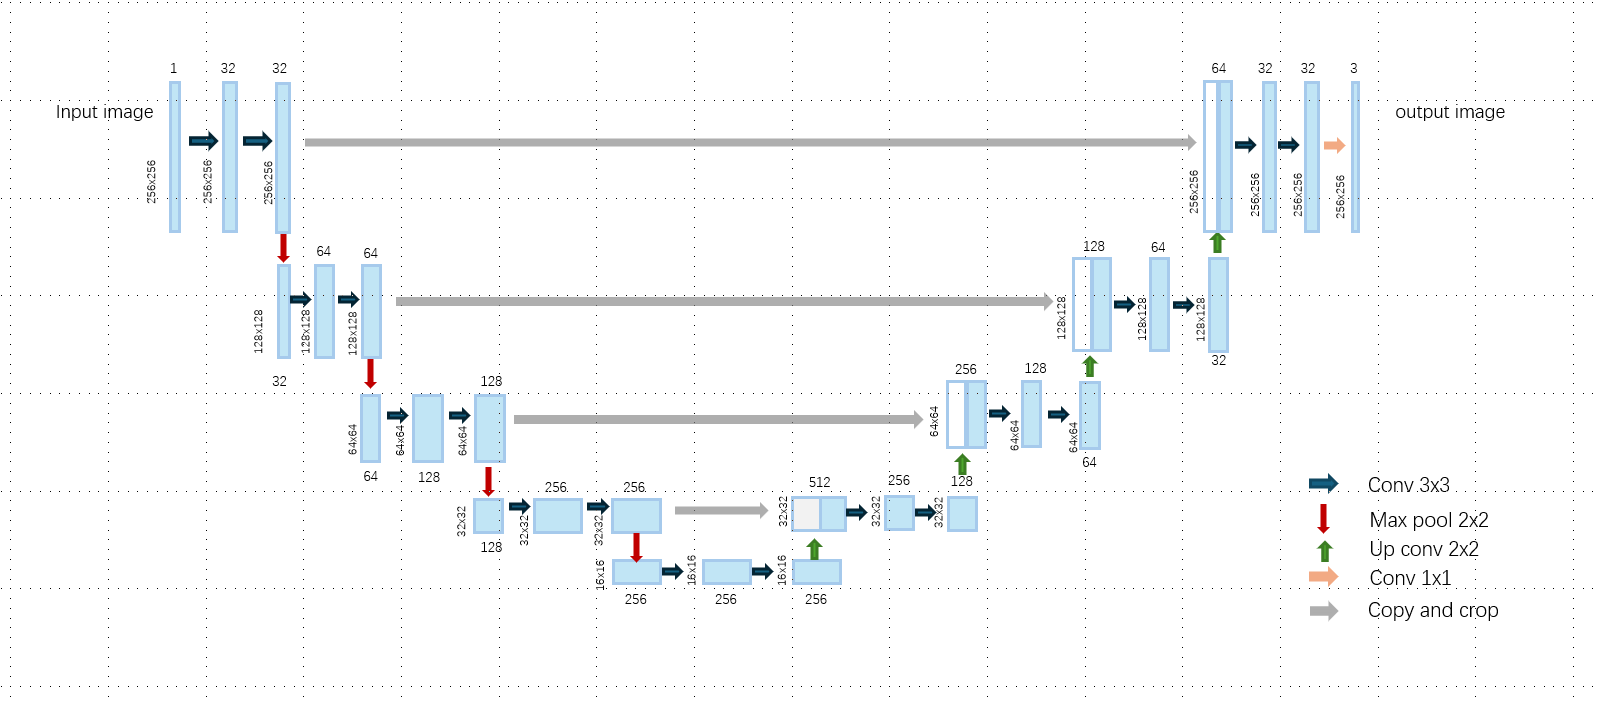
\includegraphics[width=0.8\linewidth]{../result/network.png}
  \caption{U-Net Network Architecture.}
  \label{fig:network_architecture}
\end{figure}

\subsection{Experiments and Results}
The training loss and validation loss of the baseline U-Net are shown in Figure \ref{fig:baseline_unet_loss}.
\begin{figure}[H]
  \centering
  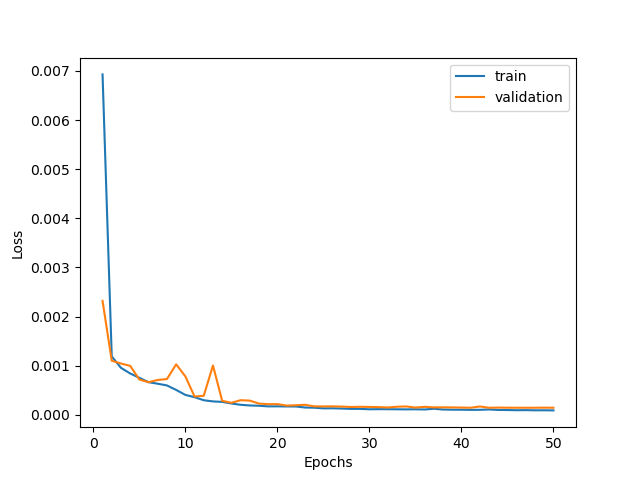
\includegraphics[width=\linewidth]{../result/baseline_unet.png}
  \caption{Training and Validation Loss Curves for the Baseline U-Net}
  \label{fig:baseline_unet_loss}
\end{figure}

And here are example segmentation results in Figure \ref{fig:baseline_unet_segmentation_example_lv},
\ref{fig:baseline_unet_segmentation_example_myo}, and \ref{fig:baseline_unet_segmentation_example_rv}.
\begin{figure}[H]
  \centering
  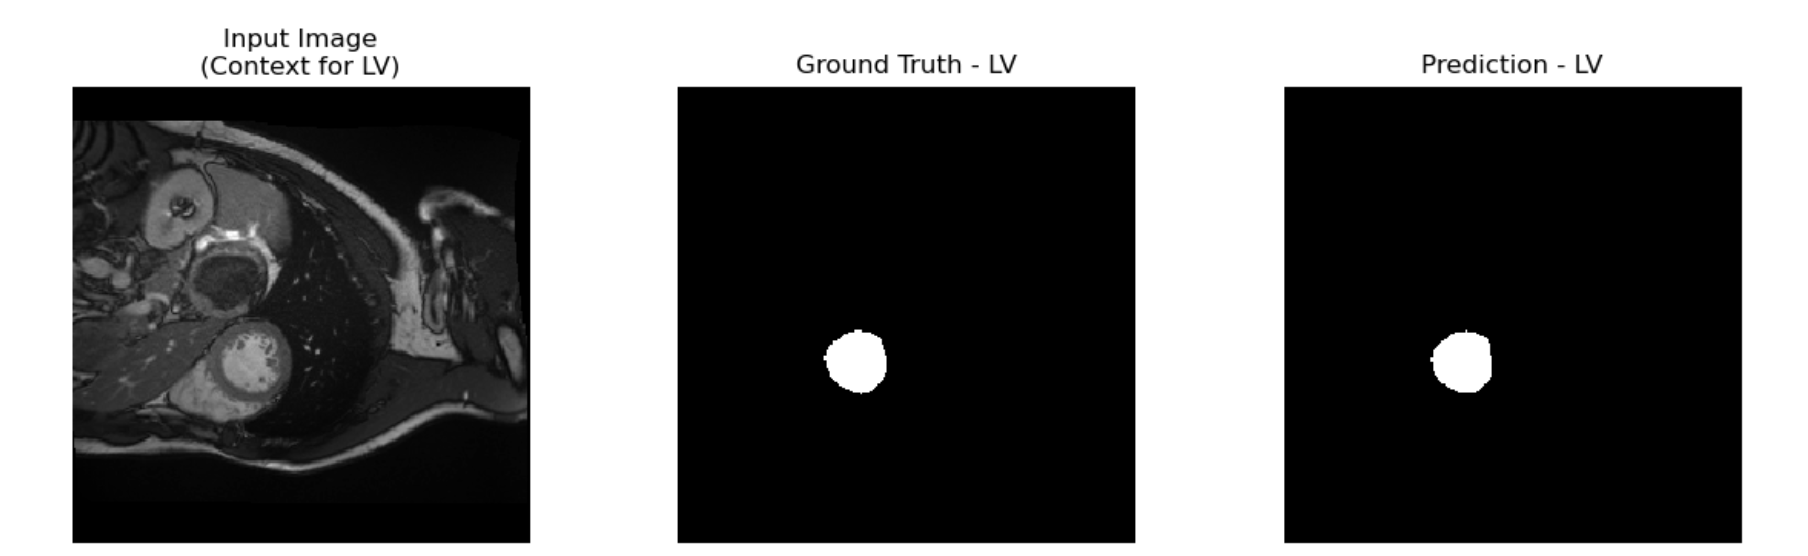
\includegraphics[width=\linewidth]{../result/for_ppt/baseline_LV.png}
  \caption{Baseline U-Net Segmentation Example: LV}
  \label{fig:baseline_unet_segmentation_example_lv}
\end{figure}
\begin{figure}[H]
  \centering
  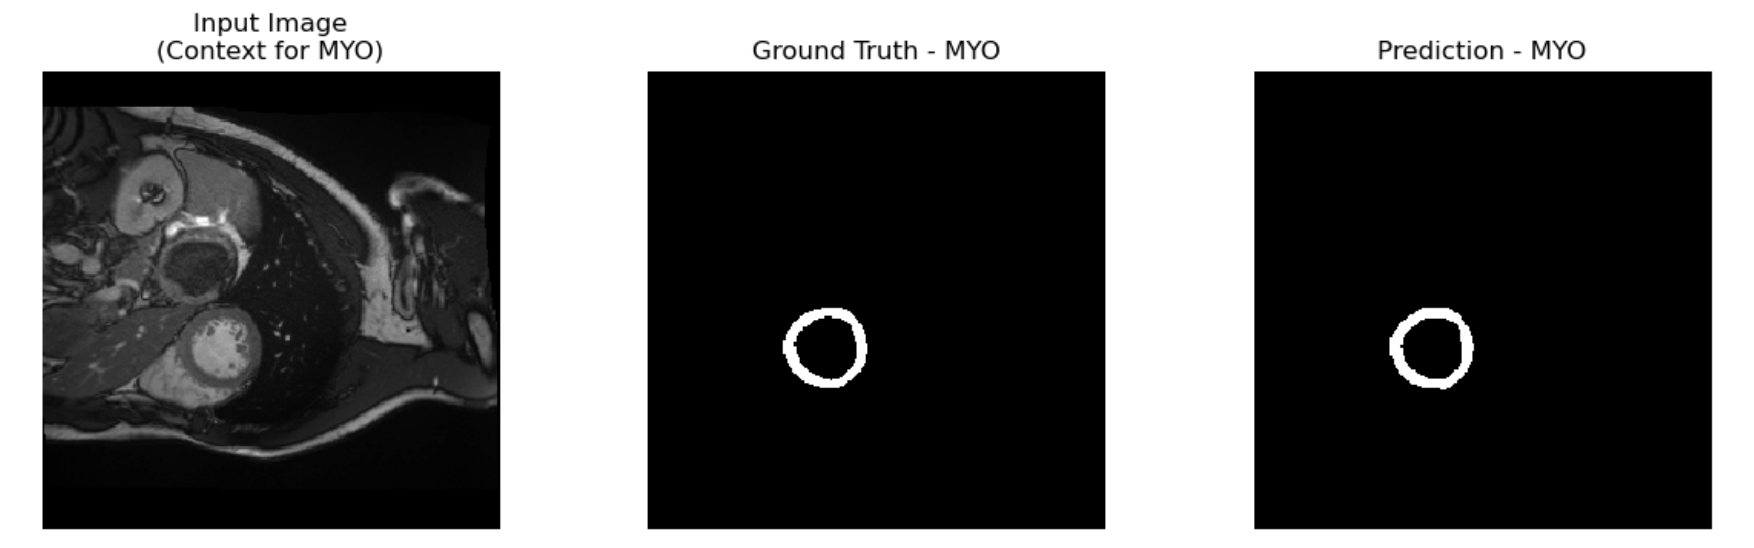
\includegraphics[width=\linewidth]{../result/for_ppt/baseline_MYO.png}
  \caption{Baseline U-Net Segmentation Example: MYO}
  \label{fig:baseline_unet_segmentation_example_myo}
\end{figure}
\begin{figure}[H]
  \centering
  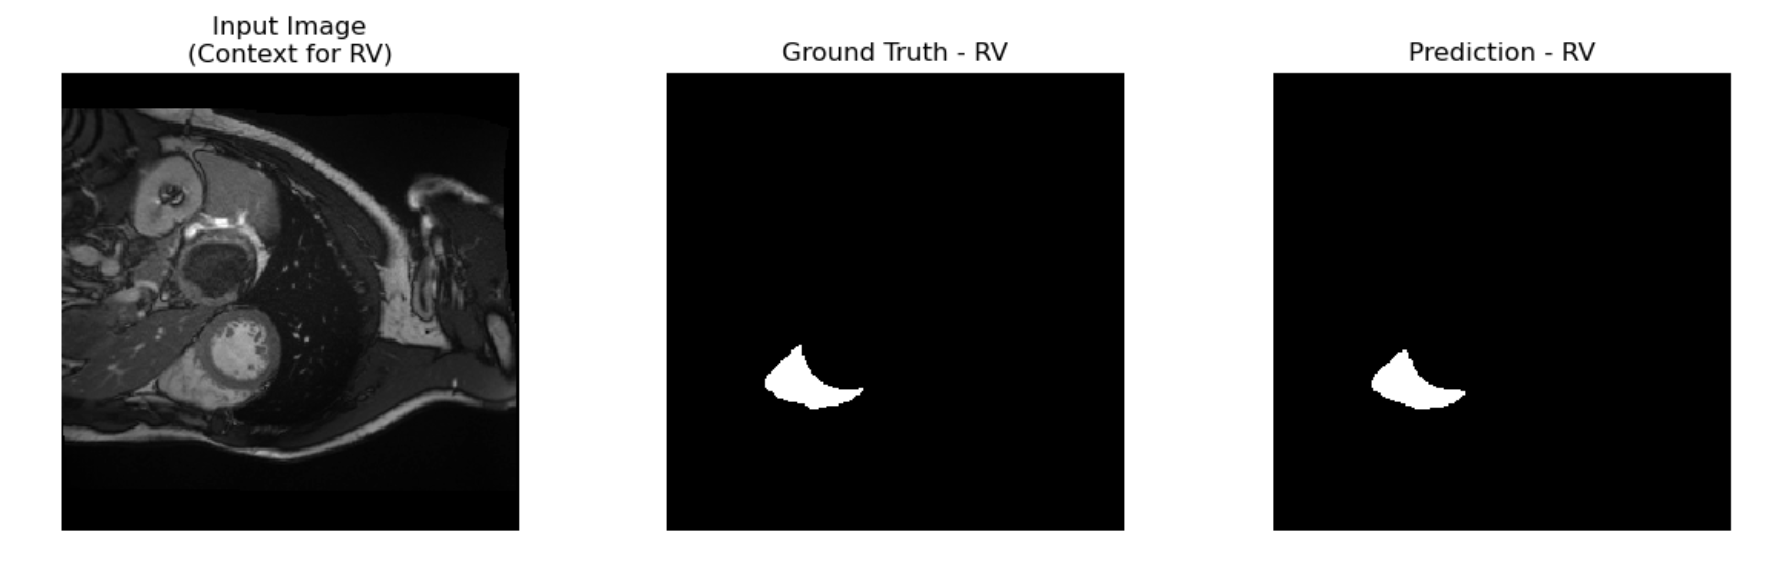
\includegraphics[width=\linewidth]{../result/for_ppt/baseline_RV.png}
  \caption{Baseline U-Net Segmentation Example: RV}
  \label{fig:baseline_unet_segmentation_example_rv}
\end{figure}

The baseline U-Net trained with Cross-Entropy loss achieved the following Dice scores (Table \ref{tab:baseline_unet}):
\begin{table}[H]
  \centering
  \caption{Dice Coefficients for Baseline U-Net (Task a)}
  \label{tab:baseline_unet}
  \begin{tabular}{lcc}
    \toprule
    Structure & Mean Dice & Standard Deviation \\
    \midrule
    RV        & 0.9519    & 0.0086             \\
    MYO       & 0.8734    & 0.0161             \\
    LV        & 0.8920    & 0.0310             \\
    \bottomrule
  \end{tabular}
\end{table}

\subsection{Discussion}
The baseline U-Net (Table \ref{tab:baseline_unet}) demonstrated strong segmentation performance.
\begin{itemize}
  \item \textbf{RV Segmentation}: Achieved the highest mean Dice score (0.9519). This is often expected as the RV is typically a large, relatively well-defined structure with good contrast against surrounding tissues in many MRI sequences.
  \item \textbf{LV Segmentation}: Also showed good performance with a mean Dice of 0.8920. The LV cavity is usually clearly visible.
  \item \textbf{MYO Segmentation}: Had the lowest mean Dice score (0.8734). The myocardium is a thinner, more complex structure surrounding the LV, and its boundaries, especially with the LV cavity (endocardium) and epicardium, can be more challenging to delineate accurately, potentially leading to lower overlap scores.
  \item The standard deviations are relatively small, indicating consistent performance across the test slices. Overall, the baseline U-Net provides a solid foundation for cardiac segmentation.
\end{itemize}


\section{U-Net without Skip Connections}

\subsection{Structure}
\begin{itemize}
  \item \textbf{Network Modification}: A \texttt{UNet\_NoShortcut} model was implemented. This involved creating an
        \texttt{Up\_NoShortcut} module that performs upsampling and convolution but does not concatenate features from the encoder
        path. The \texttt{forward} method of \texttt{Up\_NoShortcut} only processes the feature map from the previous decoder layer.
  \item \textbf{Retraining}: This modified U-Net was trained following the same procedure as the baseline U-Net: 50 epochs, Adam optimizer, learning rate of 0.01, and \texttt{MyBinaryCrossEntropy} loss.
\end{itemize}

\subsection{Performance}
The training and validation loss curves for the U-Net without skip connections are shown in Figure \ref{fig:no_shortcut_loss}.
\begin{figure}[H]
  \centering
  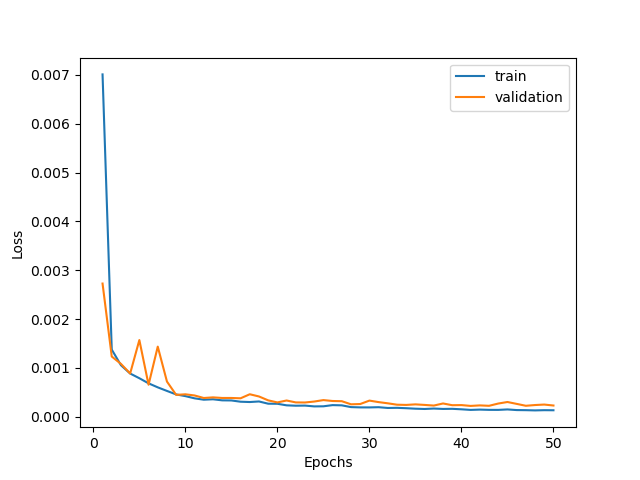
\includegraphics[width=0.8\linewidth]{../result/no_shortcut_unet.png}
  \caption{Training and Validation Loss for U-Net without Skip Connections.}
  \label{fig:no_shortcut_loss}
\end{figure}

The U-Net variant without skip connections, trained under identical conditions, yielded the Dice coefficients shown in Table \ref{tab:no_shortcut_unet_comparison}.
\begin{table}[H]
  \centering
  \caption{Dice Coefficients: Baseline U-Net vs. U-Net without Skip Connections (Task b)}
  \label{tab:no_shortcut_unet_comparison}
  \begin{tabular}{l|cc|cc}
    \toprule
    Structure & \multicolumn{2}{c|}{Baseline U-Net (DSC)} & \multicolumn{2}{c}{U-Net No Shortcut (DSC)}                         \\
              & Mean Dice                                 & Std. Dev.                                   & Mean Dice & Std. Dev. \\
    \midrule
    RV        & 0.9519                                    & 0.0086                                      & 0.9260    & 0.0111    \\
    MYO       & 0.8734                                    & 0.0161                                      & 0.8223    & 0.0168    \\
    LV        & 0.8920                                    & 0.0310                                      & 0.8588    & 0.0296    \\
    \bottomrule
  \end{tabular}
\end{table}

\subsection{Discussion}
Comparing the performance in Table \ref{tab:no_shortcut_unet_comparison}, removing skip connections resulted in a significant drop in performance across all structures.
\begin{itemize}
  \item All structures showed a noticeable decrease in Dice Similarity Coefficient (DSC).
  \item \textbf{Reason}: Skip connections provide high-resolution spatial information from the encoder to the decoder, which is crucial for accurate boundary localization. They also aid gradient flow during backpropagation, mitigating vanishing gradient problems and improving convergence.
  \item \textbf{Conclusion}: Skip connections are vital for U-Net's segmentation accuracy in this cardiac MRI segmentation task. The MYO, being the most intricate structure, suffered a substantial relative drop in performance.
\end{itemize}


\section{U-Net with Data Augmentation}

\subsection{Structure}
\begin{itemize}
  \item \textbf{Network}: The baseline U-Net architecture (with skip connections) was used.
  \item \textbf{Data Augmentation Techniques}: Augmentations were applied only to the training dataset using \texttt{torchvision.transforms}. The specific augmentations included:
        \begin{itemize}
          \item \texttt{RandomHorizontalFlip}
          \item \texttt{RandomRotation(15°)}
          \item \texttt{RandomAffine(degrees=50, translate=(0.1,0.1), scale=(0.9,1.1), shear=5)}
        \end{itemize}
        A custom \texttt{SegmentationDataset} class was used. In its \texttt{\_\_getitem\_\_} method,
        the image and its corresponding label (both single-channel tensors) were stacked along a new dimension before applying the
        transformations. This ensures that geometric augmentations are applied identically to both the image and its mask.
  \item \textbf{Retraining}: The U-Net was retrained using the augmented training data for 50 epochs.
        The validation set remained un-augmented. The loss function was \texttt{MyBinaryCrossEntropy}, and the learning rate was 0.01.
\end{itemize}

\subsection{Performance}
The training and validation loss curves for the U-Net trained with data augmentation are shown in Figure \ref{fig:data_aug_loss}.
\begin{figure}[H]
  \centering
  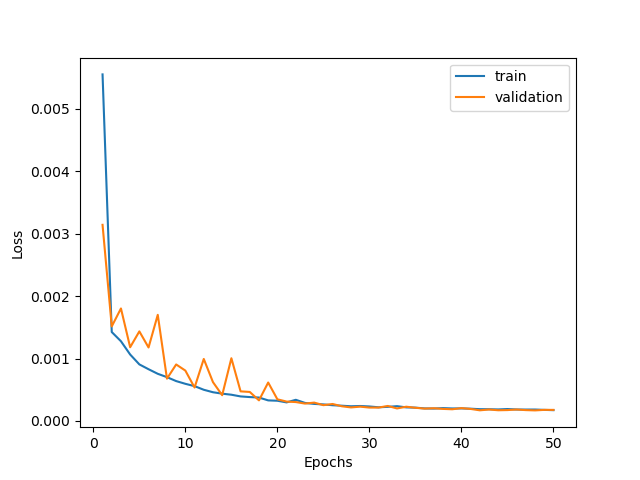
\includegraphics[width=0.8\linewidth]{../result/baseline_unet_data_aug.png}
  \caption{Training and Validation Loss for U-Net with Data Augmentation.}
  \label{fig:data_aug_loss}
\end{figure}

The baseline U-Net architecture trained with data augmentation on the training set resulted in the Dice coefficients shown in Table \ref{tab:data_aug_unet_comparison}.
\begin{table}[H]
  \centering
  \caption{Dice Coefficients: Baseline U-Net vs. U-Net with Data Augmentation (Task c)}
  \label{tab:data_aug_unet_comparison}
  \begin{tabular}{l|cc|cc}
    \toprule
    Structure & \multicolumn{2}{c|}{Baseline U-Net (DSC)} & \multicolumn{2}{c}{U-Net + Data Aug. (DSC)}                         \\
              & Mean Dice                                 & Std. Dev.                                   & Mean Dice & Std. Dev. \\
    \midrule
    RV        & 0.9519                                    & 0.0086                                      & 0.9276    & 0.0107    \\
    MYO       & 0.8734                                    & 0.0161                                      & 0.8469    & 0.0149    \\
    LV        & 0.8920                                    & 0.0310                                      & 0.8635    & 0.0384    \\
    \bottomrule
  \end{tabular}
\end{table}

\subsection{Discussion}
As shown in Table \ref{tab:data_aug_unet_comparison}, the specific data augmentation strategy employed led to a slight decrease in Dice coefficients for all structures compared to the baseline model trained on un-augmented data.
\begin{itemize}
  \item \textbf{Possible Reasons}:
        \begin{itemize}
          \item Some aggressive augmentations (e.g., large rotations or shears in \texttt{RandomAffine}) could have distorted anatomical structures or altered their relative locations significantly, making it harder for the model to learn precise boundaries.
          \item The augmentations might not be perfectly suited for the specific characteristics of cardiac MRI data, where subtle features and consistent anatomy are important.
        \end{itemize}
  \item \textbf{Conclusion}: While data augmentation is often beneficial, its effectiveness is highly dependent on the chosen transformations and the dataset. For this project, the selected augmentations did not improve performance and may have even been detrimental. More careful selection, parameter tuning, or domain-specific augmentations would be necessary to potentially see benefits.
\end{itemize}


\section{U-Net with Soft Dice Loss}

\subsection{Structure}
\begin{itemize}
  \item \textbf{Network}: The baseline U-Net architecture (with skip connections) was used.
  \item \textbf{Training Data}: The original non-augmented training dataset was used for this experiment.
  \item \textbf{Loss Function Modification}: A \texttt{SoftDiceLoss} class was implemented. This loss calculates the Dice
        coefficient directly on the sigmoid probabilities of the model's output and the multi-channel binary ground truth. The
        loss is defined as $1 - \text{mean}(\text{Dice\_per\_class})$. A smoothing factor of 1.0 was added to the numerator and
        denominator to maintain stability.
  \item \textbf{Retraining}: The U-Net model was trained for 50 epochs using the \texttt{SoftDiceLoss}. The Adam optimizer was used with a learning rate of 0.001 and an ExponentialLR scheduler.
\end{itemize}

\subsection{Performance}
The training and validation loss curves for the U-Net trained with Soft Dice Loss are shown in Figure \ref{fig:soft_dice_loss_curve}.
\begin{figure}[H]
  \centering
  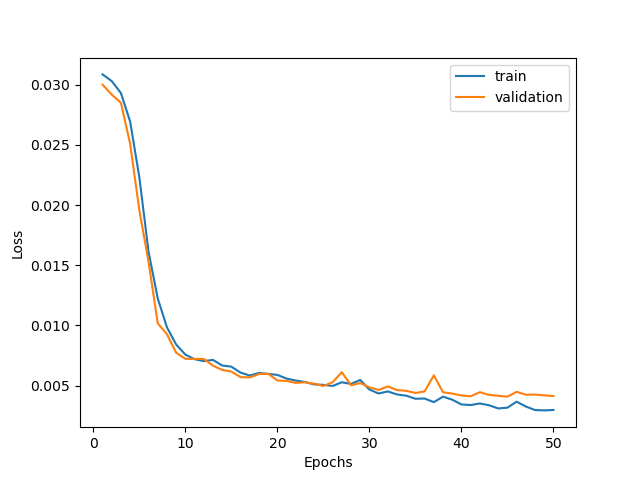
\includegraphics[width=0.8\linewidth]{../result/soft_dice_loss.png}
  \caption{Training and Validation Loss for U-Net with Soft Dice Loss.}
  \label{fig:soft_dice_loss_curve}
\end{figure}

The U-Net trained with Soft Dice Loss on the non-augmented dataset achieved the Dice coefficients shown in Table \ref{tab:soft_dice_unet_comparison}.
\begin{table}[H]
  \centering
  \caption{Dice Coefficients: Baseline U-Net (BCE Loss) vs. U-Net (Soft Dice Loss) (Task d)}
  \label{tab:soft_dice_unet_comparison}
  \begin{tabular}{l|cc|cc}
    \toprule
    Structure & \multicolumn{2}{c|}{Baseline U-Net (BCE Loss)} & \multicolumn{2}{c}{U-Net (Soft Dice Loss)}                         \\
              & Mean Dice                                      & Std. Dev.                                  & Mean Dice & Std. Dev. \\
    \midrule
    RV        & 0.9519                                         & 0.0086                                     & 0.9566    & 0.0100    \\
    MYO       & 0.8734                                         & 0.0161                                     & 0.8962    & 0.0100    \\
    LV        & 0.8920                                         & 0.0310                                     & 0.8998    & 0.0371    \\
    \bottomrule
  \end{tabular}
\end{table}

Example segmentation results for the U-Net trained with Soft Dice Loss are shown in Figures \ref{fig:soft_dice_example_lv}, \ref{fig:soft_dice_example_myo}, and \ref{fig:soft_dice_example_rv}.
\begin{figure}[H]
  \centering
  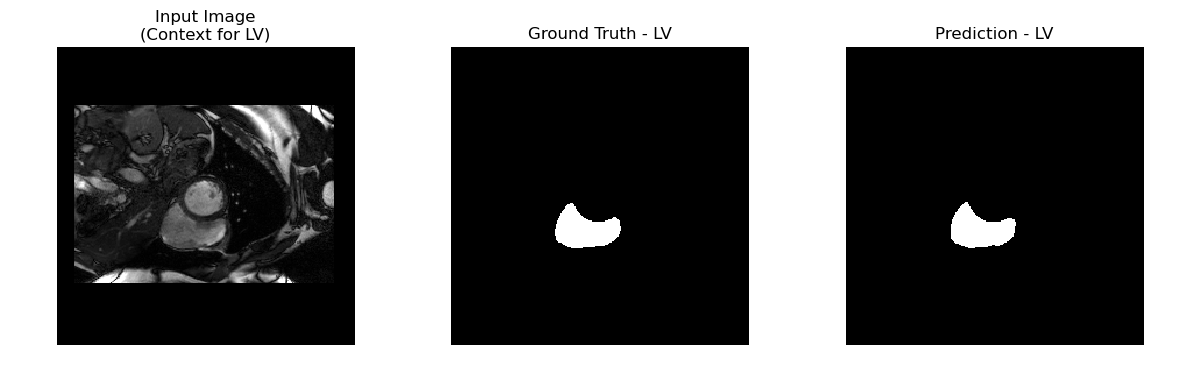
\includegraphics[width=\linewidth]{../result/for_ppt/soft_dice_loss_LV.png}
  \caption{U-Net with Soft Dice Loss Segmentation Example: LV}
  \label{fig:soft_dice_example_lv}
\end{figure}
\begin{figure}[H]
  \centering
  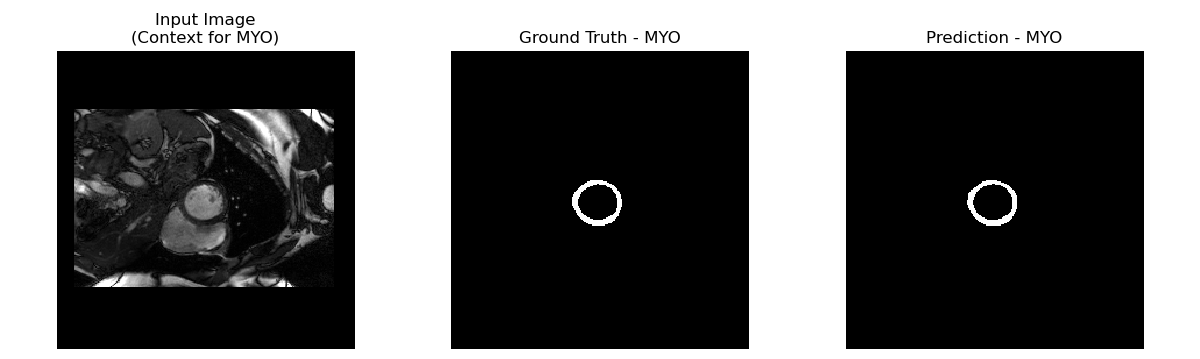
\includegraphics[width=\linewidth]{../result/for_ppt/soft_dice_loss_MYO.png}
  \caption{U-Net with Soft Dice Loss Segmentation Example: MYO}
  \label{fig:soft_dice_example_myo}
\end{figure}
\begin{figure}[H]
  \centering
  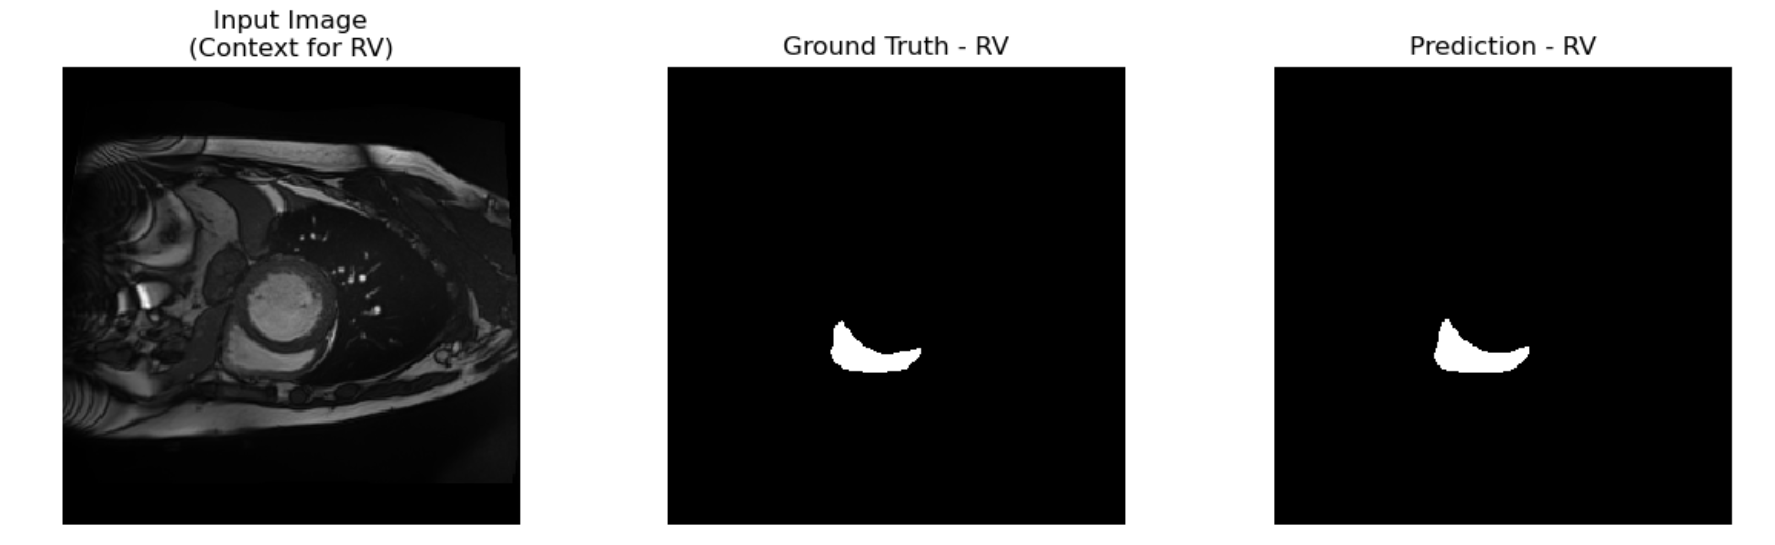
\includegraphics[width=\linewidth]{../result/for_ppt/soft_dice_loss_RV.png}
  \caption{U-Net with Soft Dice Loss Segmentation Example: RV}
  \label{fig:soft_dice_example_rv}
\end{figure}

\subsection{Discussion}
As shown in Table \ref{tab:soft_dice_unet_comparison}, when trained on the same non-augmented data, the U-Net with Soft Dice Loss significantly outperformed the baseline U-Net with Binary Cross-Entropy (BCE) Loss in terms of Dice Coefficient for all structures.
\begin{itemize}
  \item The improvement is most notable for MYO segmentation (0.8734 to 0.8962), which is often the most challenging structure.
  \item LV and RV segmentation also saw improvements.
  \item This suggests that directly optimizing a Dice-based metric is beneficial for this segmentation task, likely due to its robustness to class imbalance and focus on overlap rather than pixel-wise classification accuracy alone.
\end{itemize}


\section{Improvements: Attention U-Net}

\subsection{Structure}
To further enhance segmentation performance, an Attention U-Net architecture was implemented.
\begin{itemize}
  \item \textbf{Advanced U-Net (Attention U-Net):}
        \begin{itemize}
          \item \textbf{Architecture:} An \texttt{AttentionBlock} was introduced in the decoder's \texttt{Up} module. The \texttt{AttentionBlock} computes attention coefficients by combining features from the decoder (gating signal) and the corresponding skip connection from the encoder. These coefficients are then applied to the encoder features, effectively allowing the model to focus on more relevant spatial regions during the upsampling and feature fusion process. This helps in refining segmentation boundaries, especially for complex structures.
        \end{itemize}
  \item \textbf{Loss Function:} \texttt{SoftDiceLoss} was used, given its superior performance in the previous experiment.
  \item \textbf{Optimizer:} Adam optimizer with a learning rate of 0.001 and an ExponentialLR scheduler.
  \item \textbf{Training:} The model was trained for 50 epochs on the non-augmented training dataset.
\end{itemize}

\subsection{Performance}
The Attention U-Net trained with Soft Dice Loss achieved the Dice coefficients shown in Table \ref{tab:attention_unet_comparison}.
\begin{table}[H]
  \centering
  \caption{Dice Coefficients: Baseline (BCE), Baseline (Soft Dice Loss), and Attention U-Net (Soft Dice Loss) (Task e)}
  \label{tab:attention_unet_comparison}
  \begin{tabular}{l|cc|cc|cc}
    \toprule
    Structure & \multicolumn{2}{c|}{Baseline U-Net (BCE)} & \multicolumn{2}{c|}{U-Net (Soft Dice)} & \multicolumn{2}{c}{Attention U-Net (Soft Dice)}                                           \\
              & Mean Dice                                 & Std. Dev.                              & Mean Dice                                       & Std. Dev. & Mean Dice       & Std. Dev. \\
    \midrule
    RV        & 0.9519                                    & 0.0086                                 & 0.9566                                          & 0.0100    & \textbf{0.9588} & 0.0086    \\
    MYO       & 0.8734                                    & 0.0161                                 & 0.8962                                          & 0.0100    & \textbf{0.8967} & 0.0109    \\
    LV        & 0.8920                                    & 0.0310                                 & 0.8998                                          & 0.0371    & \textbf{0.9072} & 0.0292    \\
    \bottomrule
  \end{tabular}
\end{table}

Example segmentation results for the Attention U-Net are shown in Figures \ref{fig:attention_unet_example_lv}, \ref{fig:attention_unet_example_myo}, and \ref{fig:attention_unet_example_rv}.
\begin{figure}[H]
  \centering
  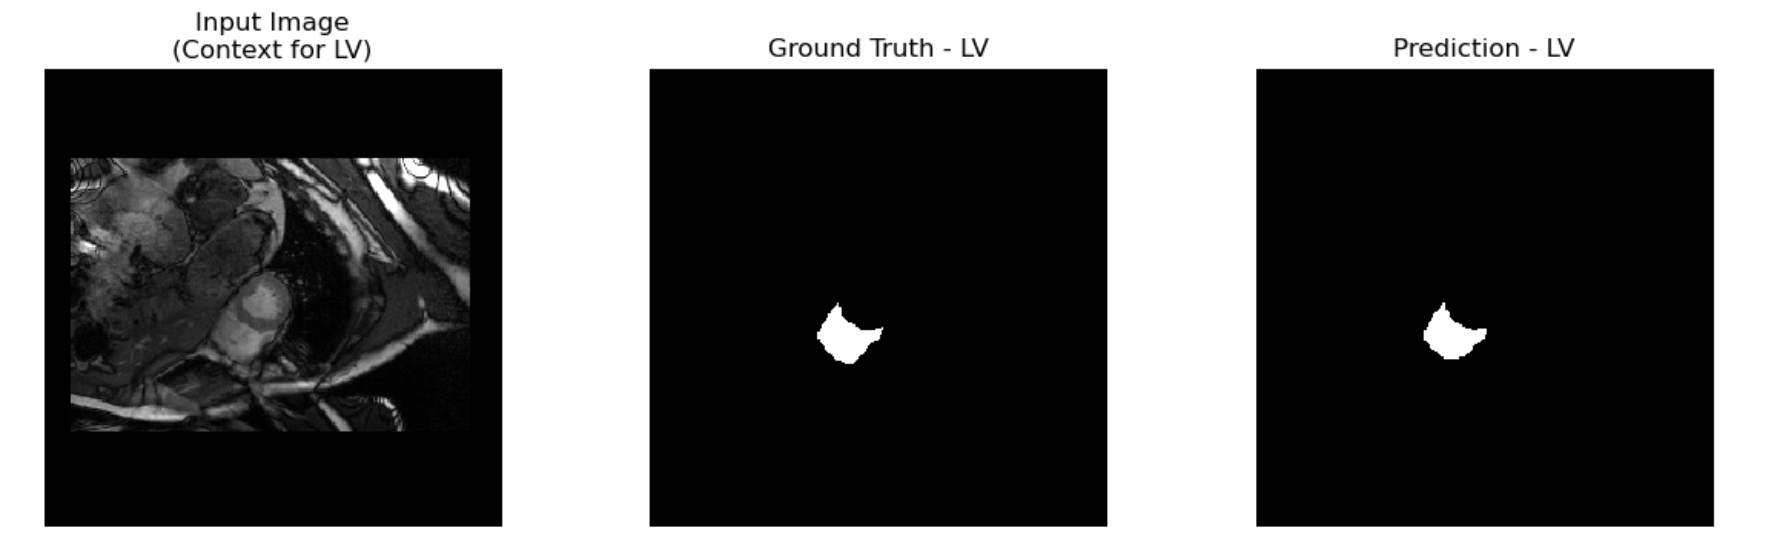
\includegraphics[width=\linewidth]{../result/for_ppt/attention_LV.png}
  \caption{Attention U-Net Segmentation Example: LV}
  \label{fig:attention_unet_example_lv}
\end{figure}
\begin{figure}[H]
  \centering
  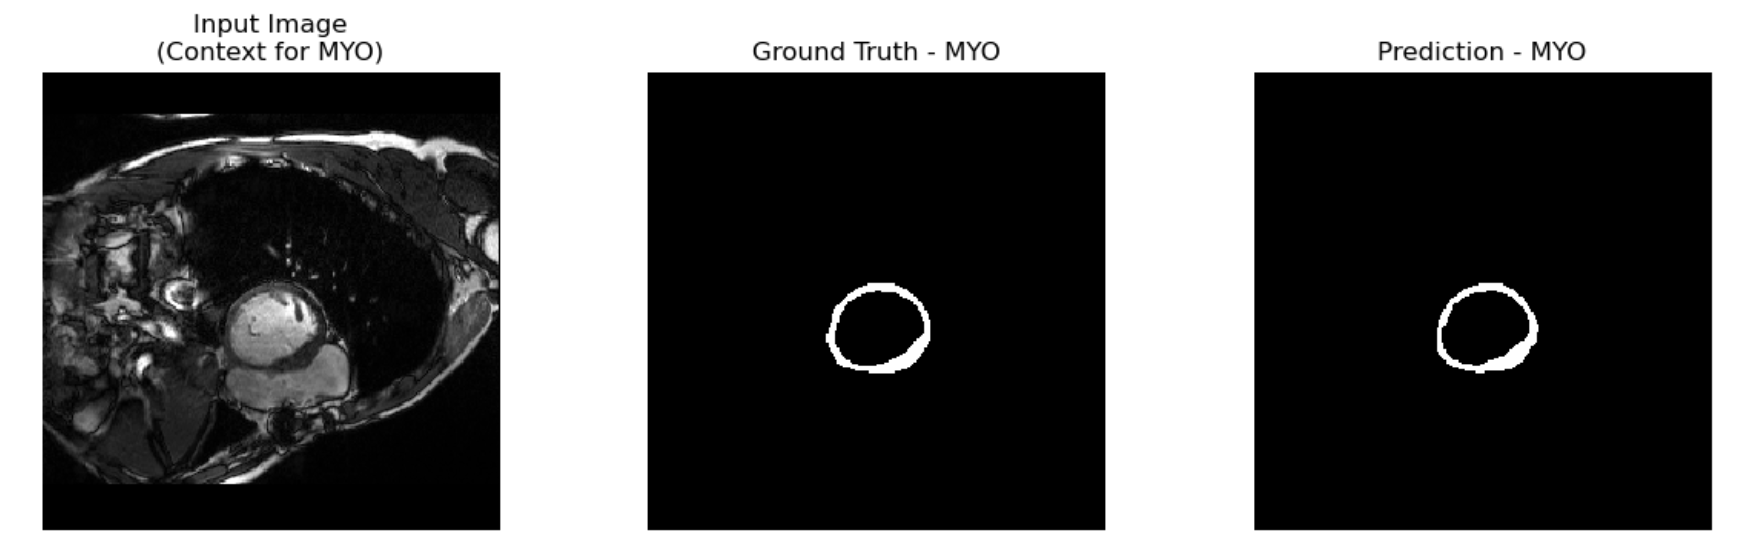
\includegraphics[width=\linewidth]{../result/for_ppt/attention_MYO.png}
  \caption{Attention U-Net Segmentation Example: MYO}
  \label{fig:attention_unet_example_myo}
\end{figure}
\begin{figure}[H]
  \centering
  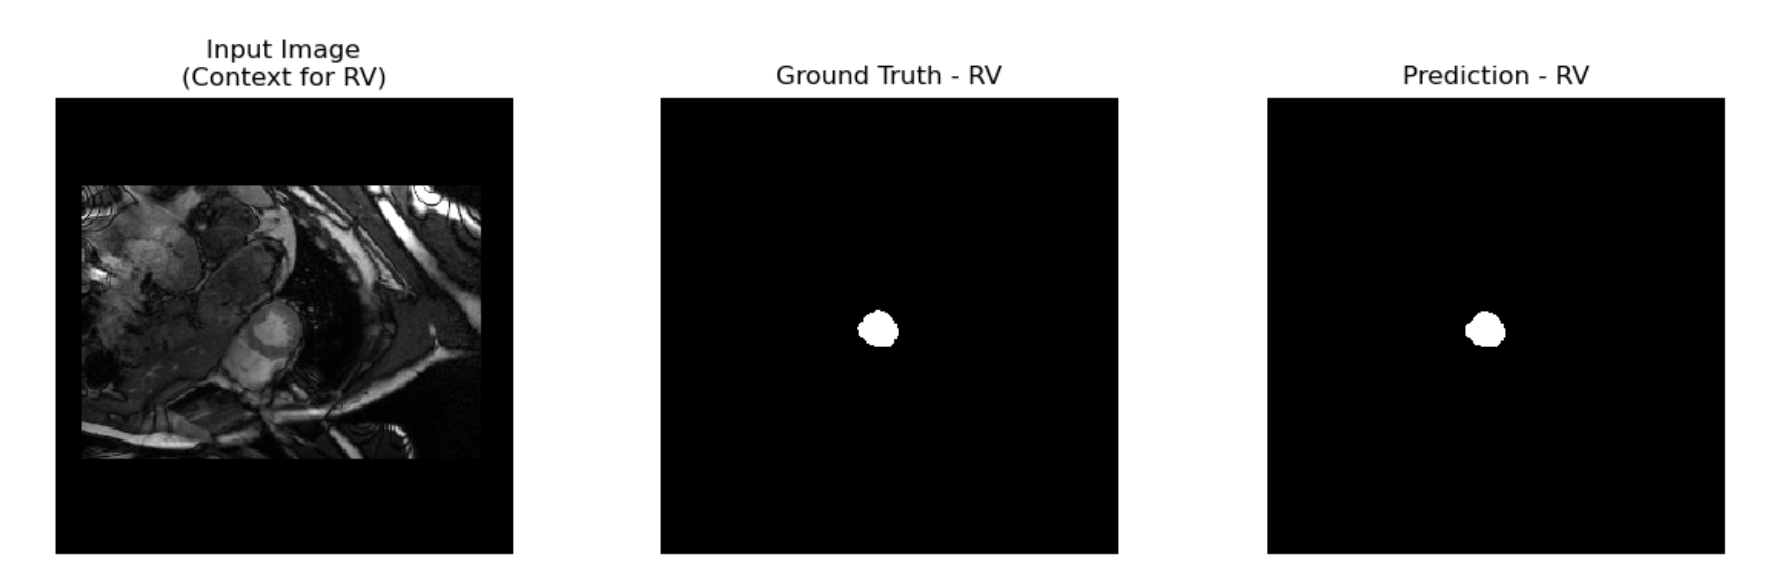
\includegraphics[width=\linewidth]{../result/for_ppt/attention_RV.png}
  \caption{Attention U-Net Segmentation Example: RV}
  \label{fig:attention_unet_example_rv}
\end{figure}

\subsection{Discussion}
The Attention U-Net, when combined with Soft Dice Loss and trained on non-augmented data, demonstrated further improvements in Dice scores compared to both the baseline U-Net with BCE loss and the U-Net with Soft Dice Loss (Table \ref{tab:attention_unet_comparison}).
\begin{itemize}
  \item The most significant improvement was observed for LV segmentation (0.8998 to 0.9072). RV and MYO also showed slight gains.
  \item This suggests that the attention mechanism effectively helps the model to focus on more salient features and complex structural details, leading to better boundary delineation and overall segmentation accuracy.
  \item The standard deviations for the Attention U-Net are comparable or slightly lower for some structures, indicating robust performance.
\end{itemize}

\section{Overall Performance Summary}
Table \ref{tab:overall_summary} provides a consolidated view of the mean Dice Similarity Coefficients (DSC) for all evaluated models across the three cardiac structures.

\begin{table}[H]
  \centering
  \caption{Overall Performance Summary: Mean Dice Coefficients}
  \label{tab:overall_summary}
  \begin{tabular}{lccc}
    \toprule
    Model Configuration                                    & RV Mean DSC     & MYO Mean DSC    & LV Mean DSC     \\
    \midrule
    (a) Baseline U-Net (BCE Loss)                          & 0.9519          & 0.8734          & 0.8920          \\
    (b) U-Net without Skip Connections (BCE Loss)          & 0.9260          & 0.8223          & 0.8588          \\
    (c) U-Net + Data Augmentation (BCE Loss)               & 0.9276          & 0.8469          & 0.8635          \\
    (d) U-Net (Soft Dice Loss, No Augmentation)            & 0.9566          & 0.8962          & 0.8998          \\
    \textbf{(e) Attention U-Net (Soft Dice Loss, No Aug.)} & \textbf{0.9588} & \textbf{0.8967} & \textbf{0.9072} \\
    \bottomrule
  \end{tabular}
\end{table}

The results clearly indicate that the Attention U-Net trained with Soft Dice Loss on the original non-augmented dataset achieved the highest performance for all three cardiac structures.


\section{Conclusion}
This project successfully implemented and evaluated several U-Net based models for cardiac cine MRI segmentation. Key findings include:
\begin{enumerate}
  \item The baseline U-Net provides a strong starting point for segmenting RV, LV, and MYO, with RV generally being the best-segmented structure.
  \item Skip connections are essential for U-Net's performance in this task. Their removal led to a significant decline in Dice scores, confirming their importance for feature reuse and precise localization.
  \item The specific data augmentation strategy employed in this study (random flips, rotations, and affine transformations) resulted in a decrease in Dice coefficients compared to training on non-augmented data. This highlights that augmentation strategies must be carefully chosen and tuned for the specific dataset and task.
  \item Training with Soft Dice Loss on non-augmented data significantly improved performance over Binary Cross-Entropy loss, particularly for the more challenging MYO structure. This indicates the benefit of directly optimizing a segmentation-specific metric.
  \item The Attention U-Net, when combined with Soft Dice Loss and trained on non-augmented data, yielded the best overall segmentation performance across all three structures (RV: 0.9588, MYO: 0.8967, LV: 0.9072). This demonstrates the effectiveness of attention mechanisms in helping the model focus on relevant features for improved boundary delineation.
\end{enumerate}
Future work could explore more sophisticated data augmentation techniques, investigate other loss functions, or experiment with different attention mechanisms or network backbones.


% \begin{figure}[H]  直方图
%   \centering
%   \begin{tikzpicture}
%     \begin{axis}
%     [ybar, 
%     grid = major, major grid style = {dashed},
%     ymin = 0,
%     ylabel = {SSIM values},
%     title = {SSIM Values for Each Model},
%     bar width = .5cm,
%     width = 40cm,
%     height = 6cm,
%     symbolic x coords={M1, M2, M3, U1, U2, U3},
%     x = 2cm,
%     xtick = data,
%     nodes near coords,
%     nodes near coords style = {font = \fontsize{8}{12}\selectfont},
%     enlarge x limits = 0.2,
%     legend style = {at = {(0.5,-0.2)},anchor = north,legend columns = -1},
%     ] 
%     \addplot+ coordinates {(M1, 0.743) (M2, 0.844) (M3, 0.844) (U1, 0.834) (U2, 0.815) (U3, 0.807)}; 
%     \addplot+ coordinates {(M1, 0.037) (M2, 0.037) (M3, 0.042) (U1, 0.030) (U2, 0.037) (U3, 0.041)}; 
%     \legend{SSIM mean, SSIM std};
%     \end{axis} 
%   \end{tikzpicture}
%   \caption{SSIM Values for Each Model}
%   \label{fig:SSIM Values for Each Model}
% \end{figure}



\end{document}